\section{Laplace Transform}
\begin{frame}{Introduction}
    \begin{itemize}
        \item Using the Fourier transform, we represented a signal as a linear combination of basic signals using the eigenfunctions $e^{j\omega t}$.
        \item Then we could represent a given LTI system as a spectrum of eigenvalues as a function of $\omega$, which is the change in amplitude that the system applies to each of the basic inputs  $e^{j\omega t}$.
        \item Now we study a generalization of the Fourier transform, referred to as the Laplace transform.
        \item The Laplace transform converges for a broader class of signals than does the Fourier transform.
    \end{itemize}
\end{frame}


\begin{frame}{The Laplace Transform}
    \begin{itemize}
        \item The general class of eigenfunctions for LTI systems consists of the complex exponential $e^{st}$, where $s$ is a complex number.
        \item When $s$ is purely imaginary, $s= j\omega$, the Laplace transform reduces to the Fourier transform.
        \item The Laplace transform is the Fourier transform of an exponentially weighted signal. Therefore, the Laplace transform can converge for signals for which the Fourier transform does not converge.
        \item The range of values of $s$  for which the Laplace transform converges is the \alert{region of convergence} (ROC).
        \item Two different signals can have Laplace transforms with identical algebraic expressions and differing only in the ROC.
    \end{itemize}
\end{frame}

\begin{frame}{Recall: Continuous-Time Fourier Transform}
    \begin{align*}
        x(t) &= \frac{1}{2\pi}\int_{-\infty}^{+\infty}X(\omega)e^{j\omega t}d\omega\\
        X(\omega) &= \int_{-\infty}^{+\infty}x(t)e^{-j\omega t}dt\\
    \end{align*}
    LTI systems: impulse response $h(t)$:
    \begin{equation*}
        \begin{matrix}
            e^{j\omega t} & \rightarrow & \quad H(\omega)e^{j\omega t} \\
            && \negthickspace\updownarrow{\mathcal{F}}\\
            && \negthickspace h(t)\\
        \end{matrix}
    \end{equation*}
\end{frame}

\begin{frame}{Laplace Transform: Eigenfunction Property}
    \begin{align*}
        e^{st} &\rightarrow \int_{-\infty}^{+\infty}h(\tau)e^{s(t-\tau)}d \tau\\
        e^{st} &\rightarrow e^{st}\int_{-\infty}^{+\infty}h(\tau)e^{-s\tau}d \tau\\
        s &= \sigma + j \omega\\
        e^{st}   &\rightarrow H(s) e^{st}\\
        H(s) &= \int_{-\infty}^{+\infty}h(\tau)e^{-s\tau}d \tau
    \end{align*}
\end{frame}


\begin{frame}{Laplace Transform}
    \begin{align*}
        X(s) &= \int_{-\infty}^{+\infty}x(t)e^{-st}dt\\
        x(t) &\xleftrightarrow{\mathcal{L}} X(s)
    \end{align*}
\end{frame}

\begin{frame}{Laplace Transform and Fourier Transform Relationship}
    \begin{align*}
        X(s) &= \int_{-\infty}^{+\infty}x(t)e^{-st}dt\\
        X(\omega) &= \int_{-\infty}^{+\infty}x(t)e^{-j\omega t}dt\\
        s &= \sigma + j\omega\\
        \left.X(s)\right|_{s=j\omega} &= \mathcal{F}\left\{ x(t)\right\}
    \end{align*}
    New notation:
    \begin{equation*}
        \mathcal{F}\left\{ x(t)\right\} = X(j\omega)
    \end{equation*}
\end{frame}

\begin{frame}{Laplace Transform: Convergence Comparison}
    \begin{align*}
        \left.X(s)\right|_{s=j\omega} &= X(j\omega)\\
        X(s) &= \int_{-\infty}^{+\infty}x(t)e^{-st}dt\\
        X(\sigma + j\omega) &= \int_{-\infty}^{+\infty}x(t)e^{-(\sigma + j\omega)t}dt\\
        &= \int_{-\infty}^{+\infty}x(t)e^{-\sigma t}e^{-j\omega t}dt\\
        X(s) &= \mathcal{F}\left\{ x(t)e^{-\sigma t}\right\}
    \end{align*}
    \uncover<2->
    {
        LT may converge when FT does not.
    }
\end{frame}

\begin{frame}[t,allowframebreaks]{}
    \begin{example}
        Find the LT of
        \begin{equation*}
            x(t) = e^{-at}u(t).
        \end{equation*}
    \end{example}

    \mode<beamer>
    {
        \begin{solution}\end{solution}
            \begin{align*}
                X(s) &= \int_{-\infty}^{+\infty}x(t)e^{-st}dt\\
                &= \int_{0}^{+\infty}e^{-at}e^{-st}dt\\
                X(s) &= \frac{1}{s+a}, \quad \mathrm{Re}\{s\} > -a\\
            \end{align*}

            \begin{equation*}
                e^{-at}u(t) \xleftrightarrow{\mathcal{L}}   \frac{1}{s+a}, \quad \mathrm{Re}\{s\} > -a
            \end{equation*}

    }

\end{frame}

\begin{frame}[t,allowframebreaks]{}
    \begin{example}
        Find the LT of
        \begin{equation*}
            x(t) = -e^{-at}u(-t).
        \end{equation*}
    \end{example}

    \mode<beamer>
    {
        \begin{solution}
            \begin{equation*}
                -e^{-at}u(-t) \xleftrightarrow{\mathcal{L}}   \frac{1}{s+a}, \quad \mathrm{Re}\{s\} < -a
            \end{equation*}
        \end{solution}
        Note: Two time functions generate the same algebraic expression for the LT. The difference is only in the ROC.
    }

\end{frame}

\begin{frame}[t]{}
    \begin{example}
        Find the LT of
        \begin{equation*}
            x(t) = e^{-t}u(t)+ e^{-2t}u(t).
        \end{equation*}
    \end{example}

    \mode<beamer>
    {

    %    \mode<beamer>
%    {
%        \begin{columns}
%            \column{0.48\textwidth}
%            \column{0.48\textwidth}
%        \end{columns}
%    }

        \begin{solution}\end{solution}
            \begin{columns}[t]
                \column[T]{0.58\textwidth}
                    \begin{align*}
                        e^{-t}u(t) &\xleftrightarrow{\mathcal{L}}   \frac{1}{s+1}, \quad \mathrm{Re}\{s\} > -1\\
                        e^{-2t}u(t) &\xleftrightarrow{\mathcal{L}}   \frac{1}{s+2}, \quad \mathrm{Re}\{s\} > -2\\
                        e^{-t}u(t)+ e^{-2t}u(t) &\xleftrightarrow{\mathcal{L}}   \frac{2s+3}{(s+1)(s+2)}, \quad \mathrm{Re}\{s\} > -1
                    \end{align*}
                    \begin{align*}
                        X(s) &= \frac{N(s)}{D(s)}\\
                        N(s) &= 0\quad \text{zeros of } X(s)\\
                        D(s) &= 0\quad \text{poles of } X(s)
                    \end{align*}

                \column[T]{0.4\textwidth}
                    \begin{tikzpicture}[scale=0.8]
    \def\pole{++(135:0.1) -- ++(-45:0.2) ++(135:0.1) -- ++(45:0.1) -- ++(-135:0.2) +(45:0.1)}
    \def\zero{circle (0.1)}
    \draw (-3, 0) -- (1,0) node[anchor=west] {$\mathrm{Re}$};
    \draw (0, -3) -- (0,3) node[anchor=south] {$\mathrm{Im}$};
    \path [pattern color=pink, pattern=north east lines] (-1, 0) ++(0,3) rectangle ++(2, -6);
    \draw (-1,0) node[anchor=north] {\scriptsize$-1$} \pole (-2, 0)  node[anchor=north] {\scriptsize$-2$}\pole (-1.5, 0) node[anchor=north] {\scriptsize $ -\frac{3}{2}$}\zero;

\end{tikzpicture} 
            \end{columns}
        %
    }
\end{frame}


\begin{frame}{Properties of the Region of Convergence}
    \begin{itemize}
        \item The ROC contains no poles
        \item The ROC of $X(S)$ consists of s trip parallel to the $j\omega$ axis in the $s$-plane.
        \item $\mathcal{F}\{x(t)\}$ converges $\Leftrightarrow$ ROC includes the $j\omega$-axis in the $s$-plane.
    \end{itemize}
\end{frame}


\begin{frame}[t]{}
    \begin{example}
        Sketch the choices of the ROC associated with
        \begin{equation*}
            X(s) = \frac{1}{(s+1)(s+2)}.
        \end{equation*}
    \end{example}
    \pause
    \mode<beamer>
    {
        \begin{solution}\end{solution}
            \begin{tikzpicture}[scale=0.6]
    \def\pole{++(135:0.1) -- ++(-45:0.2) ++(135:0.1) -- ++(45:0.1) -- ++(-135:0.2) +(45:0.1)}
    \def\zero{circle (0.1)}
    \draw (-3, 0) -- (1,0) node[anchor=west] {$\mathrm{Re}$};
    \draw (0, -3) -- (0,3) node[anchor=south] {$\mathrm{Im}$};
    \path [pattern color=pink, pattern=north east lines] (-1, 0) ++(0,3) rectangle ++(2, -6);
    \draw (-1,0)  \pole (-2, 0)  \pole ;
\end{tikzpicture}%\usetikzlibrary{patterns}
\begin{tikzpicture}[scale=0.8]
    \def\pole{++(135:0.1) -- ++(-45:0.2) ++(135:0.1) -- ++(45:0.1) -- ++(-135:0.2) +(45:0.1)}
    \def\zero{circle (0.1)}
    	%\begin{scope}
     		%\path [pattern color=pink, pattern=north east lines] (-3, -3)  rectangle (3, 3);
     		\draw [dashed, pattern color=pink, pattern=north east lines] (0,0) circle (1.5);
	%\end{scope}

    \draw (-3, 0) -- (3,0) node[anchor=west] {\scriptsize $\mathrm{Re}$};
    \draw (0, -3) -- (0,3) node[anchor=south] {\scriptsize $\mathrm{Im}$};
    %\pause
    \draw[thick, magenta] (0,0) circle (2);
    \draw [latex-] (0,0) ++(135:2) -- ++(135:0.5) node [anchor=south east] {\scriptsize Unit circle};
    \node at (2, 0) [anchor=north west] {\scriptsize $1$};

    \node at (2, 1) [anchor=west] {\scriptsize $z$-plane};
    \draw (1.5, 0) node[anchor=north east] {$a$} \pole (0,0) \zero;

\end{tikzpicture} \begin{tikzpicture}[scale=0.6]
    \def\pole{++(135:0.1) -- ++(-45:0.2) ++(135:0.1) -- ++(45:0.1) -- ++(-135:0.2) +(45:0.1)}
    \def\zero{circle (0.1)}
    \draw (-3, 0) -- (1,0) node[anchor=west] {$\mathrm{Re}$};
    \draw (0, -3) -- (0,3) node[anchor=south] {$\mathrm{Im}$};
    \path [pattern color=pink, pattern=north east lines] (-2, 0) ++(0,3) rectangle ++(-1, -6);
    \draw (-1,0)  \pole (-2, 0)  \pole ;
\end{tikzpicture}

    }
\end{frame}

\begin{frame}{ROC of a Finite-Duration Signal}
    If $x(t)$ is a finite-duration signal, then the ROC is the entire $s$-plane.

    \mode<beamer>
    {
        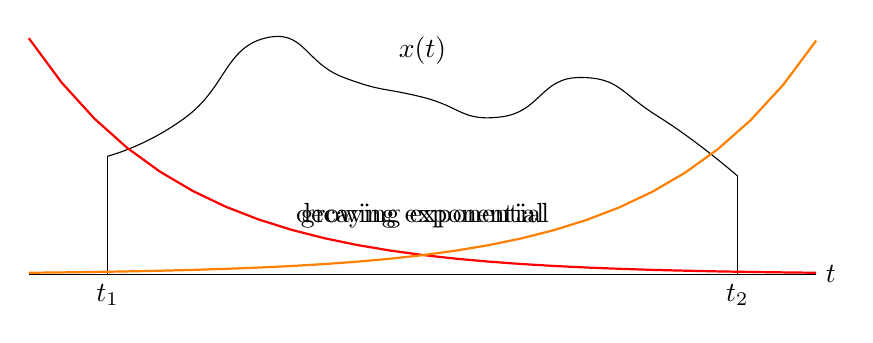
\begin{tikzpicture}[scale=1]
\draw (-5,0) -- (5,0) node[anchor=west] {$t$};
\draw  plot[smooth, tension=0.9] coordinates {(-4,1.5) (-3,2)(-2,3) (-1,2.5) (0,2.25) (1,2) (2,2.5) (3,2) (4,1.25)} node[midway, anchor=south, yshift=1in] {$x(t)$};
\draw (-4, 1.5) -- (-4, 0) node[anchor=north] {$t_1$}  (4,1.25) -- (4, 0) node[anchor=north] {$t_2$} ;
\onslide<2>
{
    \draw[thick, red,domain=0:10] plot({\x-5},{3*exp(-\x/2)}) node[midway, anchor=south, yshift=3ex, black] {decaying exponential};
}
\onslide<3->
{
    \draw[thick, orange,domain=0:10] plot({\x-5},{(exp(\x/2))/50}) node[midway, anchor=south, yshift=3ex, black] {growing exponential};
}
\end{tikzpicture} 
    }
\end{frame}


\begin{frame}{ROC of a Right-Sided Signal}
    If $x(t)$ is right-sided and $\mathrm{Re}\{s\} = \sigma_0$ is in ROC, then all values for which $\mathrm{Re}\{s\} > \sigma_0$ are in ROC.

    \mode<beamer>
    {
        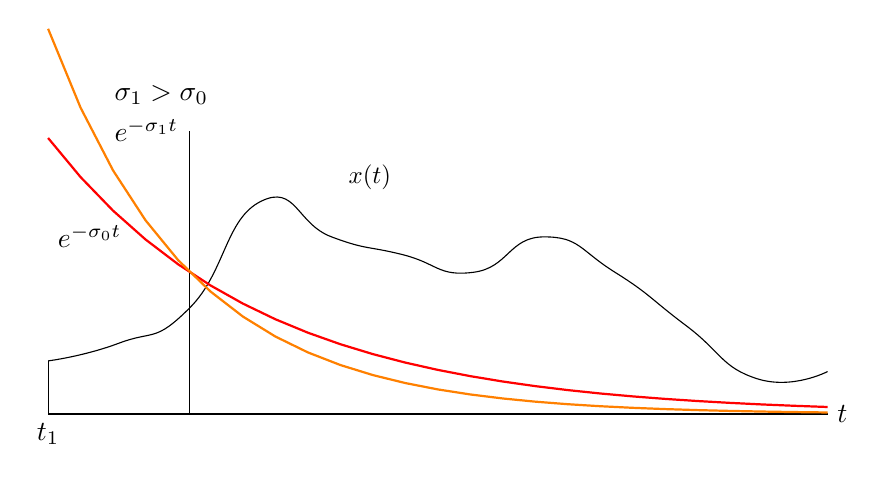
\begin{tikzpicture}[scale=0.9]
\draw (-2,0) -- (9,0) node[anchor=west] {$t$};
\draw (0,0) -- (0, 4);
\draw  plot[smooth, tension=0.9] coordinates {(-2, 0.75) (-1,1) (0,1.5)(1,3) (2,2.5) (3,2.25) (4,2) (5,2.5) (6,2) (7,1.25) (8,0.5) (9, 0.6)} node[midway, anchor=south, yshift=1.2in, xshift=1in] {$x(t)$};
\draw (-2, 0.75) -- (-2, 0) node[anchor=north] {$t_1$}  ;
\onslide<2->
{
\draw[thick, red,domain=0:11] plot({\x-2},{2*exp(-(\x-2)/3)}) ;

    \node at (-2, 2.5)  [anchor=west] {$e^{-\sigma_0 t}$};
}
\onslide<3->
{

  \draw[thick, orange,domain=0:11] plot({\x-2},{2*exp(-(\x-2)/2)});
\node at   (-1.2,4)  [anchor=west] {$e^{-\sigma_1 t}$};
    \node at (-1.2, 4.5) [anchor=west] {$\sigma_1>\sigma_0$};
}
\end{tikzpicture} 
    }

    \onslide<4->
    {
        If $x(t)$ is right-sided and $X(s)$ is rational, then ROC is the right of the rightmost pole.
    }
\end{frame}

\begin{frame}{ROC of a Left-Sided Signal}
    If $x(t)$ is left-sided and $\mathrm{Re}\{s\} = \sigma_0$ is in ROC, then all values for which $\mathrm{Re}\{s\} < \sigma_0$ are in ROC.

    %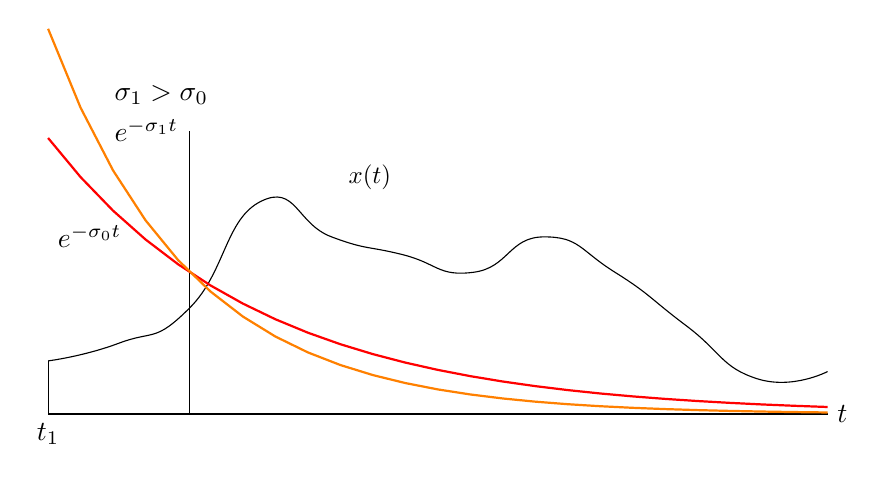
\begin{tikzpicture}[scale=0.9]
\draw (-2,0) -- (9,0) node[anchor=west] {$t$};
\draw (0,0) -- (0, 4);
\draw  plot[smooth, tension=0.9] coordinates {(-2, 0.75) (-1,1) (0,1.5)(1,3) (2,2.5) (3,2.25) (4,2) (5,2.5) (6,2) (7,1.25) (8,0.5) (9, 0.6)} node[midway, anchor=south, yshift=1.2in, xshift=1in] {$x(t)$};
\draw (-2, 0.75) -- (-2, 0) node[anchor=north] {$t_1$}  ;
\onslide<2->
{
\draw[thick, red,domain=0:11] plot({\x-2},{2*exp(-(\x-2)/3)}) ;

    \node at (-2, 2.5)  [anchor=west] {$e^{-\sigma_0 t}$};
}
\onslide<3->
{

  \draw[thick, orange,domain=0:11] plot({\x-2},{2*exp(-(\x-2)/2)});
\node at   (-1.2,4)  [anchor=west] {$e^{-\sigma_1 t}$};
    \node at (-1.2, 4.5) [anchor=west] {$\sigma_1>\sigma_0$};
}
\end{tikzpicture} 

    \onslide<2->
    {
        If $x(t)$ is left-sided and $X(s)$ is rational, then ROC is the left of the leftmost pole.
    }
\end{frame}

\begin{frame}{ROC of a Two-Sided Signal}

    %\onslide<2->
    {
        If $x(t)$ is two-sided and $\mathrm{Re}\{s\} = \sigma_0$ is in ROC, then ROC is the strip in the $s$-plane.
    }
\end{frame}


\begin{frame}[t]{}
    \begin{example}
        A Laplace transform is specified by
        \begin{equation*}
            X(s) = \frac{1}{(s+1)(s+2)}, \quad \mathrm{Re}\{s\} > -1.
        \end{equation*}
        Find the inverse laplace transform.

        \begin{tikzpicture}[scale=0.6]
    \def\pole{++(135:0.1) -- ++(-45:0.2) ++(135:0.1) -- ++(45:0.1) -- ++(-135:0.2) +(45:0.1)}
    \def\zero{circle (0.1)}
    \draw (-3, 0) -- (1,0) node[anchor=west] {$\mathrm{Re}$};
    \draw (0, -3) -- (0,3) node[anchor=south] {$\mathrm{Im}$};
    \path [pattern color=pink, pattern=north east lines] (-1, 0) ++(0,3) rectangle ++(2, -6);
    \draw (-1,0) node[anchor=north] {\scriptsize$-1$} \pole (-2, 0)  node[anchor=north] {\scriptsize$-2$} \pole;

\end{tikzpicture} 
    \end{example}
\end{frame}

\begin{frame}[t]{}
    \mode<beamer>
    {
        \begin{solution} \end{solution}
            \begin{columns}
                \column[T]{0.4\textwidth}
                    \usetikzlibrary{patterns}
\begin{tikzpicture}[scale=0.8]
    \def\pole{++(135:0.1) -- ++(-45:0.2) ++(135:0.1) -- ++(45:0.1) -- ++(-135:0.2) +(45:0.1)}
    \def\zero{circle (0.1)}
    	\begin{scope}
     		%\path [pattern color=pink, pattern=north east lines] (-3, -3)  rectangle (3, 3);
     		\draw [dashed, pattern color=pink, pattern=north east lines] (0,0) circle (2);
	\end{scope}

    \draw (-3, 0) -- (3,0) node[anchor=west] {\scriptsize $\mathrm{Re}$};
    \draw (0, -3) -- (0,3) node[anchor=south] {\scriptsize $\mathrm{Im}$};
    %\pause
    \draw[thick, magenta] (0,0) circle (1);
    \draw [latex-] (0,0) ++(135:1) -- ++(135:1.5) node [anchor=south east] {\scriptsize Unit circle};

    \node at (2, 1) [anchor=west] {\scriptsize $z$-plane};
    \draw (2, 0) node[anchor=north west] {$2$} \pole;
    \draw (1/3, 0) node[anchor=north ] {$\frac{1}{3}$} \pole;
	\draw    (0,0) \zero;
\end{tikzpicture} 
                \column[T]{0.6\textwidth}
                    \begin{align*}
                        X(s) &= \frac{1}{(s+1)(s+2)}, \quad \mathrm{Re}\{s\} > -1,\\
                        &= \frac{1}{(s+1)} - \frac{1}{(s+2)}, \quad \mathrm{Re}\{s\} > -1.
                    \end{align*}
                    \pause
                    Consider
                    \begin{align*}
                        X_1(s) &= \frac{1}{(s+1)}, \quad \mathrm{Re}\{s\} > -1,\\
                        x_1(t) &= e^{-t}u(t).
                    \end{align*}
            \end{columns}

    }
\end{frame}


\begin{frame}[t]{}
    \mode<beamer>
    {
        \begin{solution}\end{solution}
            \begin{columns}
                \column[T]{0.4\textwidth}
                    \begin{tikzpicture}[scale=0.6]
    \def\pole{++(135:0.1) -- ++(-45:0.2) ++(135:0.1) -- ++(45:0.1) -- ++(-135:0.2) +(45:0.1)}
    \def\zero{circle (0.1)}
    \draw (-3, 0) -- (1,0) node[anchor=west] {$\mathrm{Re}$};
    \draw (0, -3) -- (0,3) node[anchor=south] {$\mathrm{Im}$};
    \path [pattern color=pink, pattern=north east lines] (-1, 0) ++(0,3) rectangle ++(2, -6);
    \draw[dashed] (-2, -3) -- (-2, 3);
    \path [pattern color=orange, pattern=north west lines] (-2, 0) ++(0,3) rectangle ++(1, -6);
    \draw (-2,0) node[anchor=north] {\scriptsize$-2$} (-1,0) node[anchor=north] {\scriptsize$-1$};

\end{tikzpicture} 
                \column[T]{0.6\textwidth}
                    Consider
                    \begin{align*}
                        X_2(s) &= -\frac{1}{(s+2)}, \quad \mathrm{Re}\{s\} > -1,\\
                        x_2(t) &= -e^{-2t}u(t).
                    \end{align*}
                    So
                    \begin{equation*}
                        x(t) = (e^{-t} -e^{-2t})u(t).
                    \end{equation*}
            \end{columns}

    }
\end{frame}



\begin{frame}[t]{}
    \begin{example}
        Find the inverse laplace transform of
        \begin{enumerate}
            \item
            \begin{equation*}
                X(s) = \frac{2s+4}{s^2 + 4s+ 3}, \quad \mathrm{Re}\{s\} > -1,
            \end{equation*}
            \item
            \begin{equation*}
                X(s) = \frac{2s+4}{s^2 + 4s+ 3}, \quad \mathrm{Re}\{s\} < -3,
            \end{equation*}
            \item
            \begin{equation*}
                X(s) = \frac{2s+4}{s^2 + 4s+ 3}, \quad -3 < \mathrm{Re}\{s\} < -1,
            \end{equation*}
        \end{enumerate}
    \end{example}
\end{frame}


\begin{frame}[t]{}
    \mode<beamer>
    {
        \begin{solution}
            \begin{equation*}
                X(s) = \frac{2s+4}{s^2 + 4s+ 3} = \frac{1}{s+1} + \frac{1}{s+3}
            \end{equation*}
        \end{solution}

        \begin{enumerate}
            \item<2-> The ROC of $X(s)$ is $\mathrm{Re}\{s\} > -1$. Thus, $x(t)$ is a right-sides signal. We obtain
            \begin{equation*}
                x(t) = e^{-t}u(t) + e^{-3t}u(t) = (e^{-t}+ e^{-3t})u(t).
            \end{equation*}

            \item<3-> The ROC of $X(s)$ is $\mathrm{Re}\{s\} < -3$. Thus, $x(t)$ is a left-sides signal. We obtain
            \begin{equation*}
                x(t) = -e^{-t}u(-t) - e^{-3t}u(-t) = -(e^{-t}+ e^{-3t})u(-t).
            \end{equation*}

            \item<4-> The ROC of $X(s)$ is $-3 < \mathrm{Re}\{s\} < -1$. Thus, $x(t)$ is a double-sided signal. We obtain
            \begin{equation*}
                x(t) = -e^{-t}u(-t) + e^{-3t}u(t).
            \end{equation*}
        \end{enumerate}
    }
\end{frame}

\begin{frame}[allowframebreaks]{}
Instead of having to reevaluate the transform of a given signal, we can simply refer to the Laplace transform table and and read out the desired transform.
    \begin{center}
        \scriptsize
        \setlength{\extrarowheight}{10pt}
        \begin{longtable}{>{$}c<{$}>{$}c<{$}>{$}c<{$}}
            \toprule
            x(t) & X(s) & \text{ROC}\\
            \midrule
            \endhead
            \delta(t) & \mode<beamer>{1} & \text{All } s\\
            u(t) & \mode<beamer>{\dfrac{1}{s}} & \mathrm{Re}(s) > 0\\
            -u(-t) & \mode<beamer>{\dfrac{1}{s}} & \mathrm{Re}(s) < 0\\
            tu(t) & \mode<beamer>{\dfrac{1}{s^2}} & \mathrm{Re}(s) > 0\\
            t^ku(t) & \mode<beamer>{\dfrac{k!}{s^{k+1}}} & \mathrm{Re}(s) > 0\\
            e^{-at}u(t) & \mode<beamer>{\dfrac{1}{s+a}} & \mathrm{Re}(s) > - \mathrm{Re}(s)\\
            -e^{-at}u(-t) & \mode<beamer>{\dfrac{1}{s+a}} & \mode<beamer>{\mathrm{Re}(s) < - \mathrm{Re}(s)}\\
            te^{-at}u(t) & \dfrac{1}{(s+a)^2} & \mathrm{Re}(s) > - \mathrm{Re}(s)\\
            -te^{-at}u(-t) & \dfrac{1}{(s+a)^2} & \mathrm{Re}(s) < - \mathrm{Re}(s)\\
            \cos \omega_0t u(t) & \dfrac{s}{s^{2}+\omega^2} & \mathrm{Re}(s) > 0\\
            \sin \omega_0t u(t) & \dfrac{\omega_0}{s^{2}+\omega^2} & \mathrm{Re}(s) > 0\\
            e^{-at}\cos \omega_0t u(t) & \dfrac{s+a}{(s+a)^{2}+\omega^2} & \mathrm{Re}(s) >  - \mathrm{Re}(s)\\
            e^{-at}\sin \omega_0t u(t) & \dfrac{\omega_0}{(s+a)^{2}+\omega^2} & \mathrm{Re}(s) >  - \mathrm{Re}(s)\\
            \bottomrule
        \end{longtable}
    \end{center}
\end{frame}


\begin{frame}[allowframebreaks]{}
    \begin{center}
        \scriptsize
        \setlength{\extrarowheight}{10pt}
        \begin{longtable}{c>{$}c<{$}>{$}c<{$}>{$}c<{$}}
            \toprule
            Property & \text{Signal} & \text{Transform} & \text{ROC}\\
            \midrule
            \endhead
                & x(t) & X(s) & R\\
                & x_1(t) & X_1(s) & R_1\\
                & x_2(t) & X_2(s) & R_2\\
            Linearity & a_1x_1(t) + a_2x_2(t) &  a_1X_1(t) + a_2X_2(t)   & R^\prime \supset R_1 \cap R_2\\
            Time shifting & x(t-t_0) & \mode<beamer>{e^{-st_0}X(s)} & R^\prime = R\\
            Shifting in $s$ & e^{s_0t}x(t) & \mode<beamer>{X(s - s_0)} & R^\prime = R + \mathrm{Re}(s_0)\\
            Time scaling & x(at) & \mode<beamer>{\frac{1}{|a|}X(s)} & R^\prime = aR\\
            Time reversal & x(-t) & X(-s) &  R^\prime = -R\\
            Differentiation in $t$ & \dfrac{dx(t)}{dt} & \mode<beamer>{sX(s)} &  R^\prime \supset R\\
            Differentiation in $s$ &-tx(t) & \mode<beamer>{\dfrac{dX(s)}{ds}} &  R^\prime = R\\
            Integration & \int_{-\infty}^t x(\tau)\tau & \dfrac{1}{s}X(s) &  R^\prime \supset R \{\mathrm{Re}(s)>0\}\\
            Convolution & x_1(t) \ast x_2(t) & \mode<beamer>{X_1(s)  X_2(s)}  &   R^\prime \supset R_1 \cap R_2\\
            \bottomrule
        \end{longtable}
    \end{center}
\end{frame}



\begin{frame}{}
    \begin{example}
        Verify the time-shifting property
        \begin{equation*}
            x(t-t_0) \xleftrightarrow{} e^{-st_0}X(s), \quad R^\prime = R.
        \end{equation*}
    \end{example}
    \pause
    %\mode<beamer>
    {
        \begin{align*}
            \mathcal{L}\{x(t-t_0)\}    &= \int_{-\infty}^\infty x(t-t_0)e^{-st}dt
        \end{align*}
        By the change of variables $\tau=t-t_0$, we obtain\pause
        \begin{align*}
            \mathcal{L}\{x(t-t_0)\}    &= \int_{-\infty}^\infty x(\tau)e^{-s(\tau+t_0)}dt\\
            \pause
            &= e^{-st_0}\int_{-\infty}^\infty x(\tau)e^{-s\tau}dt\\
            &= e^{-st_0}X(s)
        \end{align*}
        with the same ROC as for $X(s)$ itself.
    }
\end{frame}

\begin{frame}[allowframebreaks]{}
    \begin{example}
        Using the various Laplace transform properties, derive the Laplace transforms of the following signals from the Laplace transform of $u(t)$.
        \begin{enumerate}
          \item $\delta(t)$
          \item $\delta^\prime(t)$
          \item $tu(t)$
          \item $e^{-at}u(t)$
          \item $te^{-at}u(t)$
          \item $\cos \omega_0t u(t)$
          \item $e^{-at}\cos \omega_0t u(t)$
        \end{enumerate}
    \end{example}
    \pause
    \mode<beamer>
    {
        \begin{enumerate}
          \item
              \begin{align*}
                \mathcal{L}\{u(t)\}    &= \int_{-\infty}^\infty u(t)e^{-st}dt\\
                &= \int_{0}^\infty e^{-st}dt\\
                &= - \left.\frac{1}{s}e^{-st}\right|_0^\infty\\
                &= \frac{1}{s}, \quad \mathrm{Re}(s)>0.
              \end{align*}
              \pause
              \begin{align*}
                \delta(t) &= \frac{du(t)}{dt}
              \end{align*}
              Thus, using time differentiation property, we obtain
              \begin{align*}
                \delta(t) &\xleftrightarrow{} {s\frac{1}{s}} = 1, \quad \text{all } s
              \end{align*}
              \pause
          \item Again applying the time-differentiation property to the result above), we obtain
              \begin{align*}
                \delta^\prime(t) &\xleftrightarrow{} s, \quad \text{all } s\\
              \end{align*}
              \pause
          \item Using the differentiation in $s$ property, we have
              \begin{align*}
                tu(t) &\xleftrightarrow{}  -\frac{d}{ds}\left(\frac{1}{s}\right) = \frac{1}{s^2}, \quad \mathrm{Re}(s)>0\\
              \end{align*}
              \pause
          \item Using the shifting in the $s$-domain property, we have
              \begin{align*}
                e^{-at}u(t) &\xleftrightarrow{}  \frac{1}{s+a}, \quad \mathrm{Re}(s)>-a\\
              \end{align*}
        \end{enumerate}

    }
\end{frame}



\section{Analysis of LTI Systems Using the Laplace Transform}

\begin{frame}{Introduction}
    \begin{itemize}
        \item The properties of the Laplace transform make it useful in analyzing LTI systems that are represented by linear constant-coefficient differential equations.
        \item Applying the Laplace transform to a differential equation converts it to an algebraic equation relating the Laplace transform of the system output to the product of the Laplace transform of the system input and the Laplace transform of the system impulse response, referred to as the system function.
        \item The system function is readily obtained by inspection of the differential equation, and the system impulse response can be obtained by evaluating the inverse Laplace transform of the system function.
        \item Alternatively, the response for any other input can be evaluated by first multiplying the Laplace transform of the input by the system function and then applying the inverse Laplace transform.
    \end{itemize}
\end{frame}

\begin{frame}{First- and Second-Order Systems}
    \begin{itemize}
        \item Two particularly important classes of systems described by linear constant-coefficient differential equations are first-order and second-order systems.
        \item In implementing higher-order systems, it is very common to use first and second-order systems as building blocks.
        \item First-order systems are represented by a single pole in the $s$-plane, and second-order systems by a pair of poles. There may or may not also be zeros in the transfer function, depending on whether there are derivative terms on the right-hand side of the differential equation.
        \item From the differential equation, the system function can be written directly.
        \item If we assume that the systems are causal, so that the impulse response is right-sided, then the ROC of the system function is implicitly specified to be to the right of the rightmost pole in the $s$-plane.
    \end{itemize}
\end{frame}

\begin{frame}{Recall: Laplace Transform}
    \begin{align*}
        X(s) &= \int_{-\infty}^{+\infty}x(t)e^{-st}dt\\
        x(t) &\leftrightarrow X(s)\\
        \left.X(s)\right|_{s=j\omega} &= X(j\omega) = \mathcal{F}\left\{ x(t)\right\}\\
        s &= \sigma + j\omega\\
         X(s) &= \mathcal{F}\left\{ x(t)e^{-\sigma t}\right\}
    \end{align*}
    LT converges for some values of $\sigma$ and not others: ROC.
\end{frame}


\begin{frame}{Properties}
    \begin{equation*}
        ax_1(t) + bx_2(t) \xleftrightarrow{\mathcal{L}} aX_1(s) + bX_2(s).
    \end{equation*}

    \begin{equation*}
        \frac{dx(t)}{dt} \xleftrightarrow{\mathcal{L}} sX(s).
    \end{equation*}
    \begin{center}
        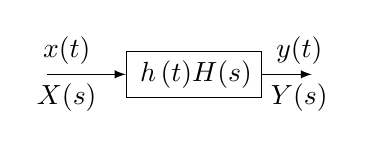
\begin{tikzpicture}
	\draw[-latex] (0,0) --++(1,0) node[near start, above] {$x(t)$} node[near start, below]  {$X(s)$} node[draw, anchor=west] (sys) {$\begin{matrix}h(t)\\H(s)\end{matrix}$};
	\draw[-latex] (sys) -- ++(1.5,0)  node[near end, above] {$y(t)$} node[near end, below]  {$Y(s)$};
\end{tikzpicture}
    \end{center}


    \begin{equation*}
        Y(s) = H(s)X(s).
    \end{equation*}

    Stable, causal $\Leftrightarrow$ all poles in left-half $s$-plane
\end{frame}

\begin{frame}{First-Order System}
    \begin{equation*}
        \begin{matrix}
            \dfrac{dy(t)}{dt} & +& ay(t) &= &x(t)\\
            \pause
            \downarrow &&\downarrow &&\downarrow\\
            \pause
            sY(s) & +& aY(s) &= &X(s)\\
        \end{matrix}
    \end{equation*}
    \pause
\mode<beamer>
{
    \begin{align*}
        Y(s) &= \dfrac{1}{s+a}X(s), \quad \mathrm{Re}\{s\}>a\\
        h(t) &\xleftrightarrow{\mathcal{L}} H(s)
    \end{align*}
    \pause
    \begin{align*}
        e^{-at}u(t) &\xleftrightarrow{\mathcal{L}} \dfrac{1}{s+a}, \quad \mathrm{Re}\{s\}>-a\\
        e^{-at}u(-t) &\xleftrightarrow{\mathcal{L}} \dfrac{1}{s+a}, \quad \mathrm{Re}\{s\}<-a
    \end{align*}
}
\end{frame}

\section{Continuous Time Second Order Systems}

\begin{frame}[t]{Second-Order System}
    \begin{columns}[t]
        \begin{column}{6cm}
            \begin{equation*}
                \dfrac{d^2y(t)}{dt^2} + 2\zeta\omega_n\dfrac{dy(t)}{dt} + \omega_n^2y(t) = \omega_n^2x(t).
            \end{equation*}
            \pause
            \mode<beamer>
            {
                \begin{equation*}
                    \left[s^2 + 2\zeta\omega_ns + \omega_n^2\right]Y(s) = \omega_n^2X(s).
                \end{equation*}
            }
            \pause
            \mode<beamer>
            {
                \begin{equation*}
                    H(s) = \dfrac{\omega_n^2}{s^2 + 2\zeta\omega_ns + \omega_n^2}.
                \end{equation*}
            }
            \pause
            \mode<beamer>
            {
                \begin{equation*}
                    H(s) = \dfrac{\omega_n^2}{(s - c_1)(s - c_2)}.
                \end{equation*}
            }

        \end{column}
        \begin{column}{4cm}
            \mode<beamer>
            {
                \begin{equation*}
                    c_1 =\pause -\zeta\omega_n + \omega_n\sqrt{\zeta^2 - 1}
                \end{equation*}
            }
            \vspace{-0.2in}
            \mode<beamer>
            {
                \begin{equation*}
                    c_2 =\pause -\zeta\omega_n - \omega_n\sqrt{\zeta^2 - 1}
                \end{equation*}
            }
            For $\zeta < 1$,
            \begin{equation*}
                \begin{split}
                    c_1&=c_2^\ast\\
                    &= -\zeta\omega_n + j\omega_n\sqrt{1-\zeta^2}\\
                \end{split}
            \end{equation*}

        \end{column}
    \end{columns}

\end{frame}

\begin{frame}
    \begin{center}
        \begin{tikzpicture}[scale=1.2]
	\def\al{3}
   	 \def\pole{++(135:0.1) -- ++(-45:0.2) ++(135:0.1) -- ++(45:0.1) -- ++(-135:0.2) ++(45:0.1)}
    	\def\zero{circle (0.1)}
	\tikzstyle{helper} = [orange,thick, dashed]    	
	\coordinate (o) at (0,0);
	\draw (-\al,0) -- (\al,0) node[anchor=west] {$\mathrm{Re}$};
	\draw (0, -\al) -- (0,\al) node[anchor=south] {$\mathrm{Im}$};
\mode<beamer>
{
    \draw[red, thick] (o) ++(120:2) \pole;
    \draw[red, thick] (o) ++(-120:2) \pole;
    \node at (2.5, 2) [anchor=south] {$0<\zeta<1$};
    \pause
	\draw[helper] (o) -- ++(30:2.5);
	\draw[helper] (o) -- ++(120:2)    -- ++(0,-2*0.866) node[anchor=north, text=black] {$-\zeta \omega_n$};	
	\draw[helper, latex-latex] (o) ++(120:2) -- ++(30:2.5) ++(-150:0.1) -- ++(-60:2) node[midway, fill=white, , text=black] {$\omega_n$};
	\draw[helper] (o) ++(120:2) --++(1, 0) node[anchor=west, text=black] {$\omega_n\sqrt{1-\zeta^2}$};
	\draw[helper] (o) ++(-0.5,0) arc (180:120:0.5);
	\node at (-0.3, -0.05) [anchor=south] {$\theta$};
	\node at (1.2, 0.0) [anchor=south] {$\cos\theta = \zeta$};
}
	

\end{tikzpicture} 
    \end{center}
\end{frame}

\begin{frame}
    \begin{center}
        \begin{tikzpicture}[scale=1.2]
	\def\al{3}
   	 \def\pole{++(135:0.1) -- ++(-45:0.2) ++(135:0.1) -- ++(45:0.1) -- ++(-135:0.2) ++(45:0.1)}
    	\def\zero{circle (0.1)}
	\tikzstyle{helper} = [orange,thick, dashed]    	
	\coordinate (o) at (0,0);
	\draw (-\al,0) -- (\al,0) node[anchor=west] {$\mathrm{Re}$};
	\draw (0, -\al) -- (0,\al) node[anchor=south] {$\mathrm{Im}$};
\mode<beamer>
{
	\draw[red, thick] (-0.2,0) \pole ;

	\node at (2.5, 2) [anchor=south] {$\zeta>1$};	
	\draw[red, thick] (-1.8, 0) \pole;
	
	\draw[helper] (-0.2, 0) -- ++(0, 1);
	\draw[helper] (-1.8, 0) -- ++(0, 1);	
	\draw[helper, latex-latex] (-0.2, 0.9) -- ++(-1.6, 0) node[midway, above, text=black] {$2\omega_n\sqrt{\zeta^2 - 1}$};	
	\draw (-1, 0.1) -- ++(0, -0.2)  ++(0,0.1) node[anchor=north] {$-\zeta\omega_n$};
}
\end{tikzpicture} 
    \end{center}
\end{frame}



\begin{frame}[plain,t]
    %\mode<beamer>
    {
    \begin{figure}
      \centering
      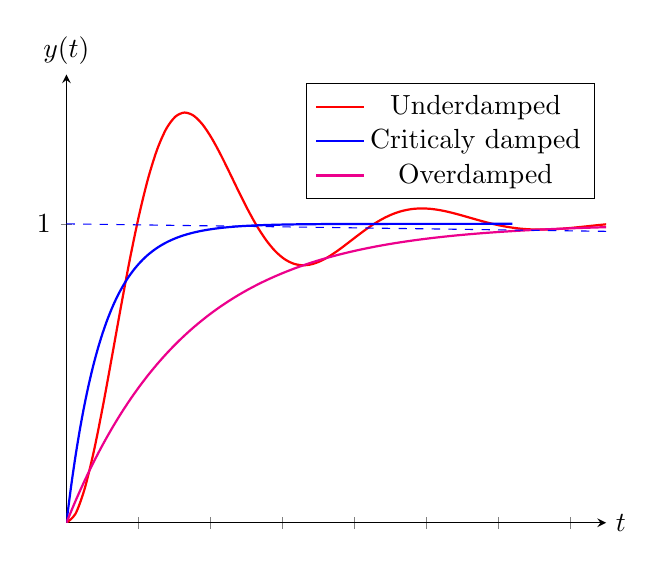
\begin{tikzpicture}
% https://tex.stackexchange.com/questions/312523/step-response-in-tikz
\begin{axis}[
        axis lines=middle,
        xmin=0, xmax=15,
        ymin=0, ymax=1.5,
        xlabel=$t$,
        ylabel={$y(t)$},
        xlabel style={at=(current axis.right of origin), anchor=west},
        ylabel style={at=(current axis.above origin), anchor=south},
        %xtick={0, 0.4726, 1.79398, 1.96605, 3.2236, 11.0855},
        %xticklabels={$0$, $t_{r_1}$, $t_{r_1}$, $t_r$, $t_p$, $t_s$},
        xticklabels = none,
        %ytick={0, 0.1, 0.9, 1, 1.3714},
        %yticklabels={$0$, $0.1$, $0.9$, $1$, $M_p$}
        ytick = {0,1},
        yticklabels = {0,1},
    ]
    \addplot[smooth, 
             red,
             thick,
             mark=none,
             domain=0:25,
             samples=100]
    {1-exp(-0.3*x)*(cos(deg(sqrt(1-0.3^2)*x))+0.3/(sqrt(1-0.3^2))*sin(deg(sqrt(1-0.3^2)*x)))};
    
    \addplot[smooth, 
             blue,
             thick,
             mark=none,
             domain=0:12.4,
             samples=100] {1-exp(-1*x)};
             
     \addplot[smooth, 
             magenta,
             thick,
             mark=none,
             domain=0:25,
             samples=100] {1-exp(-0.3*x)};
    %
%     \addplot[black, dotted] coordinates{(0.4726,0.1)} -- (axis cs:0,0.1);
%     \addplot[black, dotted] coordinates{(0.4726,0.1)} -- (axis cs:0.4726,0);
%     %
%     \addplot[black, dotted] coordinates{(1.79398,0.9)} -- (axis cs:0,0.9);
%     \addplot[black, dotted] coordinates{(1.79398,0.9)} -- (axis cs:1.79398,0);
%     %
%     \addplot[black, dotted] coordinates{(1.96605,1)} -- (axis cs:1.96605,0);
%     %
%     \addplot[black, dotted] coordinates{(3.2236,1.3714)} -- (axis cs:0,1.3714);
%     \addplot[black, dotted] coordinates{(3.2236,1.3714)} -- (axis cs:3.2236,0);
%     %
%     \addplot[black, dotted] coordinates{(11.0855,1.025)} -- (axis cs:11.0855,0);
%     %
%     \addplot[black, thick] coordinates{(15,0.9872)} -- (axis cs:12.4,0.9872);
%     %
%     \addplot[black, dashed] coordinates{(15,1)} -- (axis cs:0,1);
%     %
	 \addplot[blue, dashed] coordinates{(15,0.975)} -- (axis cs:0,1);
%     \addplot[blue, dashed] coordinates{(15,1.025)} -- (axis cs:0,1.025);

    %\coordinate (a) at (axis cs:0,0);
    %\coordinate (b) at (axis cs:1.79398,0);
	\legend{Underdamped,Criticaly damped, Overdamped},
    \end{axis}

    %\draw [shorten <=1mm,shorten >=1mm] (a) -- ++(0,-1cm) coordinate (aa);
    %\draw (b) -- ++(0,-1cm) coordinate (bb);
    %\draw [|<->|] (aa) -- (bb) node [midway,fill=white] {$t_r$};

    \end{tikzpicture}
      \caption{Second-order system responses.}\label{fi:second_order_response}
    \end{figure}
    }
\end{frame}

\begin{frame}
    \begin{example}
        The transfer function of a network is
        \begin{equation*}
            H(s) = \frac{s+10}{s^2+4s+8}
        \end{equation*}
        Determine the pole-zero plot of $H(s)$, the type of damping exhibited by the network, and the unit step response of the.
    \end{example}
    \pause
    \mode<beamer>
    {
        Solution: The network is underdamped.\\
        \pause
        \begin{equation*}
          y(t) = \left[\frac{10}{8}+1.4e^{-2t}\cos(2t-210.96^\circ)\right]u(t)
        \end{equation*}
    }
\end{frame}

\begin{frame}
    \begin{example}
        Consider an $RLC$ series network.
        \begin{circuitikz}[scale=1]
%--------start graphics code --------
%\draw[step=0.5,very thin,black!20] (-1,-0.5) grid (6,2.5);
\path (0,0) coordinate (ref_gnd);
\draw
  (ref_gnd) to[/tikz/circuitikz/bipoles/length=1cm, american voltage source=\(v_{i}(t)\)] ++(0,2)
            to[/tikz/circuitikz/bipoles/length=1cm, R=\(R\)] ++(3,0)
            to[/tikz/circuitikz/bipoles/length=1cm, L=\(L\)] ++(3,0)
            to[/tikz/circuitikz/bipoles/length=1cm, C, l_={\(C\)}, v^<=$v_{o}(t)$] ++(0,-2)
  -- (ref_gnd);
%--------end graphics code ----------
\end{circuitikz}
\begin{enumerate}
    \item Obtain the voltage transfer function.
    \item If $\omega_n = 2000\:\mathrm{rad/s}$ and $zeta=0.25, 0.50, 0.75$, and $1.0$, sketch the pole-zero plots.
    \item Sketch the step response for each case.
\end{enumerate}
    \end{example}
\end{frame}


\section{The Unilateral Laplace Transform}

\begin{frame}{Introduction to The Unilateral Laplace Transform}
    \begin{itemize}
      \item In the preceding sections, we have dealt with what is commonly called the bilateral Laplace transform.
      \item In this section, we briefly study the unilateral Laplace transform.
      \item  It is of considerable value in analyzing causal systems and, particularly, systems specified by linear constant-coefficient differential equations with nonzero initial conditions (i.e., systems that are not initially at rest).
    \end{itemize}

\end{frame}


\begin{frame}{The Unilateral Laplace Transform}
    \begin{equation*}
        \mathcal{X}(s) \triangleq \int_{0^{-}}^{\infty}x(t)e^{-st}dt
    \end{equation*}
    where the lower limit of integration, $0^{-}$, signifies that we include in the interval of integration any impulses or higher order singularity functions concentrated at $t = 0$.
    \begin{equation*}
        x(t) \xleftrightarrow{\mathcal{UL}} \mathcal{X}(s)
    \end{equation*}

    \pause
    \mode<beamer>
    {
    \begin{tikzpicture}[remember picture,overlay]  \node at (current page.east) [anchor=east, text width=2in, fill=pink]{    $X(s) = \int_{-\infty}^{+\infty}x(t)e^{-st}dt$\\ $x(t) \xleftrightarrow{\mathcal{L}} X(s)$}; \end{tikzpicture}
    }

    The system analysis tools and system function algebra developed and used in this lecture apply without change to unilateral transforms, \alert{as long
as we deal with causal LTI systems (for which the system function is both the bilateral and the unilateral transform of the impulse response) with inputs that are identically zero
fort $t< 0$}.
\end{frame}



\begin{frame}
    \begin{example}
        A causal LTI system is described by the differential equation
        \begin{equation*}
            \frac{d^2y(t)}{dt^2} + 5\frac{dy(t)}{dt} + 6y(t) = x(t).
        \end{equation*}
        Suppose that the system is at initial rest.
        \begin{enumerate}
            \item Find the system function $\mathcal{H}(s)$.
            \item Find the Laplace transform of the output $\mathcal{Y}(s)$ if the input is $x(t) = \alpha u(t)$.
            \item Find the output $y(t)$.
        \end{enumerate}
    \end{example}
\end{frame}





\begin{frame}
    \mode<beamer>
    {
        \begin{equation*}
            \frac{d^2y(t)}{dt^2} + 3\frac{dy(t)}{dt} + 2y(t) = x(t).
        \end{equation*}
        System function is
        \begin{equation*}
            \mathcal{H}(s) = \frac{1}{s^2 + 3s + 1}
        \end{equation*}
        \pause
        \begin{align*}
          x(t) &= \alpha u(t)\\
          X(s) &= \alpha \frac{1}{s}\\
        \end{align*}
        \pause
        \begin{equation*}
            \begin{split}
            \mathcal{Y}(s) &=  \mathcal{H}(s)\mathcal{X}(s) = \frac{\alpha}{s(s^2 + 3s + 1)}\\
            &= \frac{\alpha/2}{s} - \frac{\alpha}{s+1} +\frac{\alpha/2}{s+2}
            \end{split}
        \end{equation*}
        \pause
        \begin{equation*}
            y(t) = \alpha \left[ \frac{1}{2} - e^{-t} + \frac{1}{2}e^{-2t}\right]u(t)
        \end{equation*}

    }
\end{frame}

